\chapter{HW watermarking}
Nowadays, the development of integrated circuits has moved to an intellectual propriety paradigm, 
instead of the traditional manufacturing paradigm of building everything from scratch.
This means that most of the complexity of the development problem has became mainly putting together
different blocks of IP cores.\\
Furthermore, those IPs can be provided from the source in different formats: the designer of the IP can provide
the layout of the component to be integrated in the final design, without providing the details of the
implementation(\textit{hard IP}), or the HDL model of the component(\textit{soft IP}).\\
Because of the shift of the development paradigm, one has to trust the IP provider, because the IP can be
vulnerable to different kind of attacks, such as reverse engineering, piracy, and counterfeiting.
\begin{boxH}
  \textbf{Watermarking} means \textbf{adding a signature} to the integrated circuit such that its 
  very difficult to discover the functioning an replicating it without being found out.
\end{boxH}

The watermark must not:
\begin{itemize}
  \item be easy to remove
  \item alter the functionalities of the IP(duh)
  \item degrade performance
  \item leak informations
\end{itemize}
It has also to be verifiable by the owner of the IP.\\
Watermarking is also used in different domains, such as multimedia, where some pixels are usually altered 
to embed the watermark. Of course this is not possible in the case of ICs.\\
For ICs, there are two main families of watermarking: \textbf{static} and \textbf{dynamic}.
\begin{section}{Static Watermarking}
  Static watermarking add a signature in the IC, but verifying it is very difficult, because it 
  is very intrusive and expensive(microscopic analysis), so its not very used, and only for very 
  profitable IPs.\\
  Because we cannot influence performance or altering the functionality, some constraints can act 
  as a watermark. As such, we can model the watermark as a constraint satisfaction problem, where the 
  constraints act as the watermark itself.
  We also add several signature, such as we have a lot of constraints to be satisfied, making the 
  watermark "stronger", because the CSP is NP-hard.\\
  The CSP can be modelled as follows: assume $C$ constraints are integrated, each with probability 
  $p$ of being satisfied.
  Then let $X$ be a random variable that represent how many constraints are not satisfied, then 
  the probability to have $b$, or less, constraints not satisfied is
  \begin{equation}
    P(X\le b )=\sum^b_{i=0}\binom{C}{i}p^{C-i}\cdot(1-p)^i
  \end{equation}
  Furthermore, those constraints can be added at different levels of the design.

  \begin{subsection}{System level watermarking}
    With system level watermarking, the constraints are added at the system level, which means that
    the watermark is the schedule of the operations.\\ 
    Imagine that a series of operations have to be scheduled in different time slots. For example, in
    figure \ref{fig:syslevelwm}, we have some operations to be scheduled over 4 time slots.
    \begin{figure}[H]
      \centering
      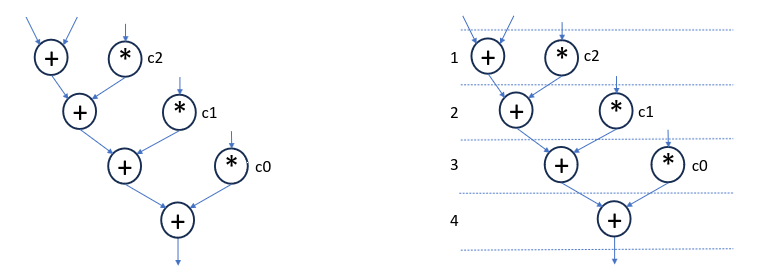
\includegraphics[width=0.7\textwidth]{img/hardware/system level watermarking.png}
      \caption{A series of task scheduled over 4 time slots.}
      \label{fig:syslevelwm}
    \end{figure}
    Those ones can can be scheduled in different ways, for example one can anticipate each of them 
    at different times to obtain a different schedule, without altering the functionalities.\\
    \begin{figure}[H]
      \centering
      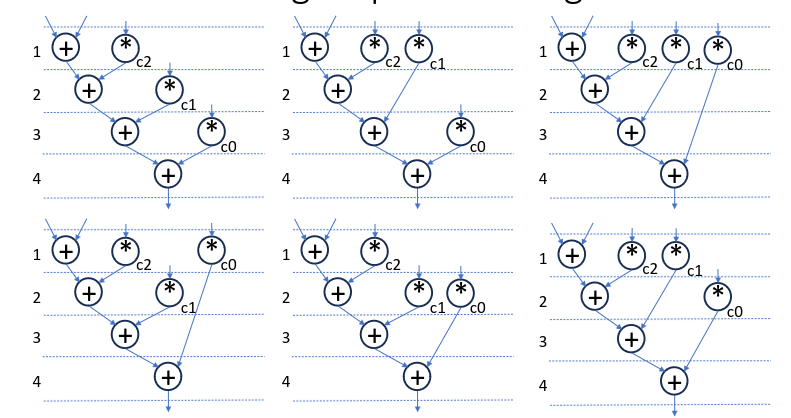
\includegraphics[width=0.6\textwidth]{img/hardware/system level watermarking 2.png}
      \caption{Different ways to schedule the tasks in figure \ref{fig:syslevelwm}.}
      \label{fig:syslevelwm2}
    \end{figure}
  \end{subsection}
  
  \begin{subsection}{Register allocation}
    We can also embed the watermark at a lower level, such as the register allocation.\\
    Any algorithm produces intermediate results, and those results can be stored in different registers,
    and are going to be used at different times, having different lifetime. As such, we can find out how
    many registers are needed, because they can be used at different times by different variables.
    We can model the association between the variables and the registers as a graph, and the constraints
    of the watermark are those of a graph coloring problem, meaning the watermark is the coloring of the graph.\\
    For example, in figure \ref{fig:graphcoloring}, we have a graph that represents the association between
    variables and registers. For example $v_1$ is connected to $v_{12}$, $v_{14}$, $v_{16}$ and $v_{18}$.
    \begin{figure}[H]
      \centering
      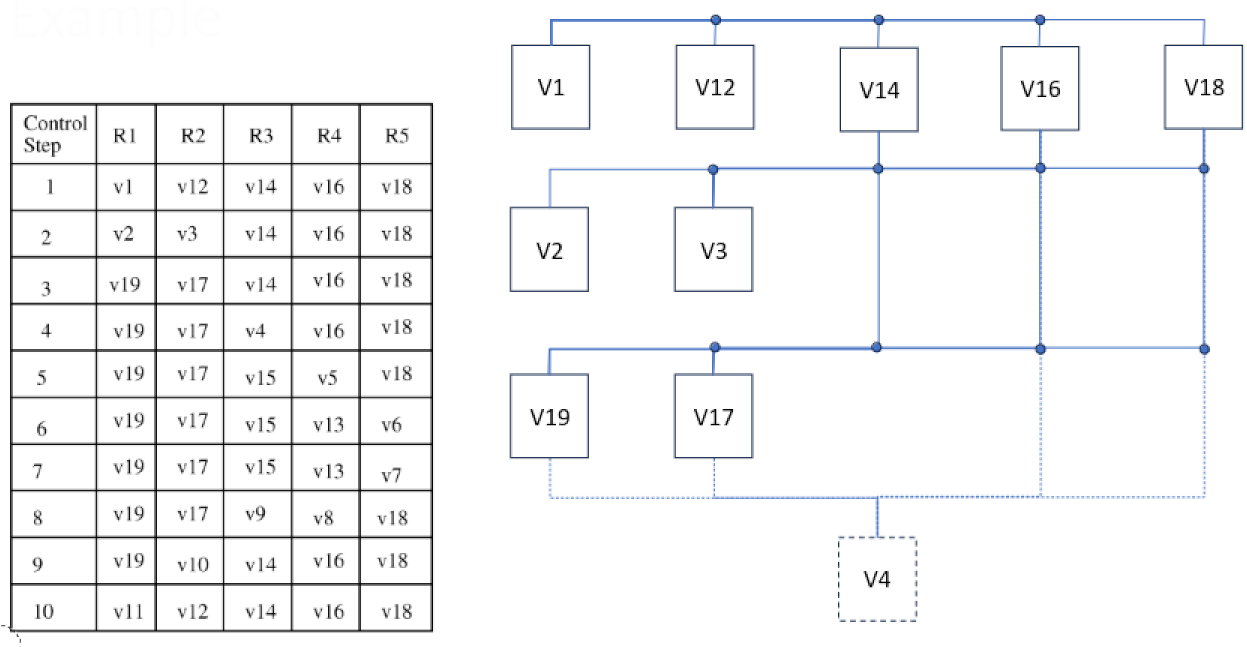
\includegraphics[width=0.6\textwidth]{img/hardware/register allocation.png}
      \caption{A example of an association between variables and registers.}
      \label{fig:graphcoloring}
    \end{figure}
    To color the graph, we need 5 colors, and we can add constraints to fix the colouring strategy,
    by adding edges between the nodes in a specific order.
    For example, we can sort the nodes in increasing duration order and then decide to embed a 0 if 
    if we have a new connection to an even node, and 1 otherwise.
    Now, imagine that we want to add the signature 10000010110111 to the graph. 
    The sorted nodes are $v_1,v_2,v_3,v_4,v_5,v_6,v_7,v_8,v_9,v_{10},v_{11},v_{12}$, so for the first step 
    we want to add a 1, so we have to add the connection $v_1\to v_3$, because its the next odd node by 
    order of duration.\\
    The second step is to add a 0, so we have to add the connection $v_2\to v_4$, because its the next
    even node by order of duration, and so on and so forth.\\ 
    The result can be something like the one in figure \ref{fig:graphcoloring2}. Of course, its not 
    the only possible one, if not, the watermark could not be possible to be verified.
    \begin{figure}[H]
      \centering
      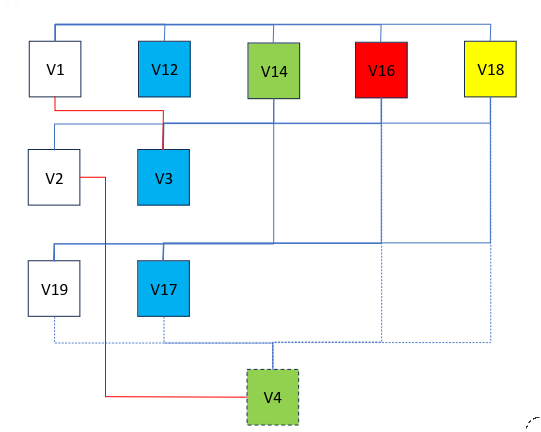
\includegraphics[width=0.4\textwidth]{img/hardware/register allocation 2.png}
      \caption{A possible colouring of the graph in figure \ref{fig:graphcoloring}.}
      \label{fig:graphcoloring2}
    \end{figure}
  \end{subsection}

  \begin{subsection}{Logic synthesis watermarking}
    We can also embed the watermark at the logic synthesis level.\\
    The logic synthesis is the process of transforming the HDL code into a netlist, and the constraints
    can be added at this level.\\
    To embed at synthesis level we have to be careful not to decrease performance.\\
    We exploit the fact that when we are performing the logic synthesis we have a constraint at the 
    maximum clock frequency, so we have a path in the whole design that complies with the requirement,
    because otherwise it would reduce the performance.\\
    To comply with this requirement, we can work on the non-critical paths, because they are not going
    to affect the performance.\\
    We can work with a mapping approach, called \textit{K-M-macrocell}, where the logic minimization is
    already done, and physical cells, or standard blocks, have at most $K$ inputs and $M$ outputs.\\
    \begin{figure}[H]
      \centering
      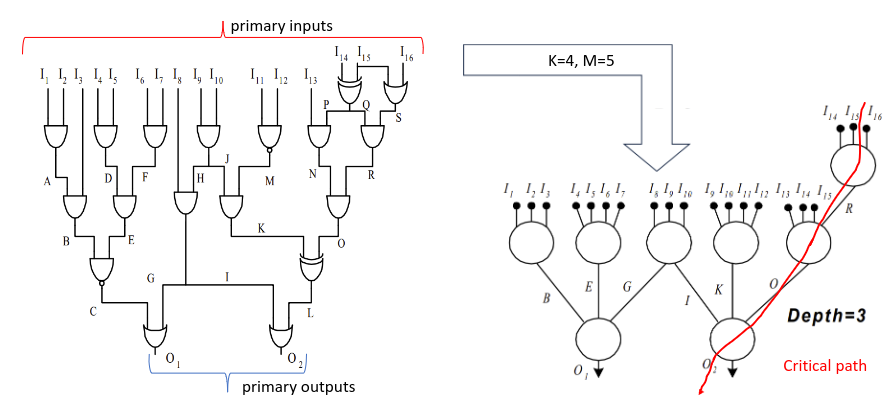
\includegraphics[width=0.6\textwidth]{img/hardware/mapping watermarking.png}
      \caption{A logic circuit that has to be mapped}
      \label{fig:K-M-macrocell}
    \end{figure}
    The nodes can be mapped with K-M-macrocells, assigned a label to each of them. This mapping can 
    then be removed from the nodes in which the watermark will be encoded, except for the nodes that 
    are going to be used in the critical path, while also breaking the selected signals in pairs 
    of primary inputs and outputs.\\
    Then, the mapping can be performed again, to obtain a different mapping.
    \begin{figure}[H]
      \centering
      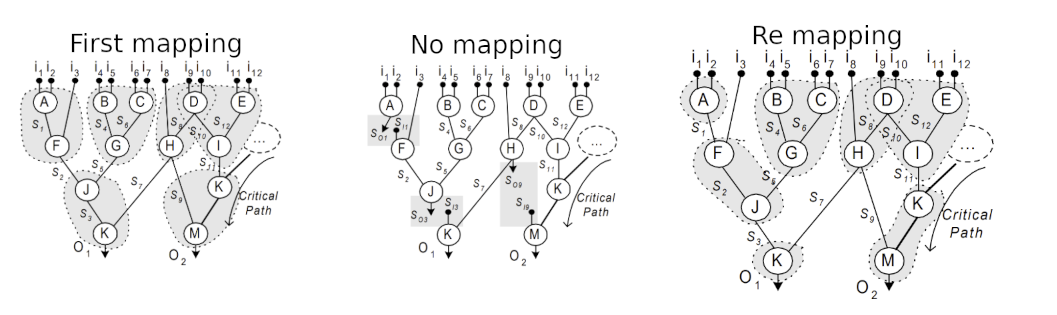
\includegraphics[width=0.8\textwidth]{img/hardware/mapping watermarking 2.png}
      \caption{The remapping of the circuit in figure \ref{fig:K-M-macrocell}.}
      \label{fig:K-M-macrocell2}
    \end{figure}
  \end{subsection}

  \begin{subsection}{Physical synthesis level}
    We can also embed the watermark at the physical synthesis level.\\
    If we want a FPGA design, we can use the unused blocks as a signature. In case of ASIC, we can watermark
    the layout of certain cells for a subset of the core.
  \end{subsection}


\end{section}
